\documentclass{article}
\usepackage{a4wide}
\usepackage{anysize}
\usepackage{latexsym}
\usepackage{amsmath}
\usepackage{amssymb}
\usepackage{epsfig}
\usepackage{tabls}
\usepackage[dvips]{color}
\usepackage{fullpage}
\usepackage{times}
\usepackage{tabularx}

\usepackage{algorithm}
\usepackage[noend]{algorithmic}

\newcommand{\cI}{{\cal I}}
\newcommand{\cM}{{\cal M}}
\newcommand{\cN}{{\cal N}}
\newcommand{\RR}{{\mathbb R}}
\newcommand{\OPT}{\operatorname{OPT}}

%\marginsize{2cm}{2cm}{2cm}{2cm}

%\linespread{1.6}
\newcommand{\ignore}[1]{}

\newtheorem{theorem}{Theorem}
\newtheorem{fact}{Fact}
\newtheorem{conjecture}{Conjecture}
\newtheorem{lemma}{Lemma}
\newtheorem{corollary}{Corollary}
\newtheorem{claim}{Claim}
\newtheorem{definition}{Definition}
\def\tab{\hspace{5mm}}
\newenvironment{proof}{\medskip\noindent {\bf Proof.}}{~\hfill$\Box$\medskip}
%\def\proof{\noindent {\bf Proof:}\hspace{2mm}}
%\def\claim{\noindent \textbf{Claim}}
\def\bsq{$\blacksquare$}
\def\sse{\subseteq}



\newcommand{\todo}[1]{TODO: \uppercase{#1}}

\title{Algorithm for Online K-Means Clustering}

\author{
	Edo Liberty \thanks{Yahoo Labs, New York, NY}
		\and
	Ram Sriharsha \thanks{Yahoo Labs, Sunnyvale, CA}
       		\and 
	Maxim Sviridenko \thanks{Yahoo Labs, New York, NY}
}



\begin{document}


\date{}
\maketitle{}
\mbox{}
\begin{abstract}
This paper shows that one can be competitive with with the $k$-means objective while operating online.
In this model, the algorithm receives vectors $v_1,\ldots,v_n$ one by one in arbitrary order. 
For each vector $v_i$ the algorithm outputs a cluster identifier before receiving $v_{i+1}$.
Our online algorithm generates $\tilde{O}(k)$ clusters whose $k$-means cost is $\tilde{O}(W^*)$ where $W^*$ is the optimal $k$-means cost using $k$ clusters.\footnote{The notation $\tilde{O}(\cdot)$ depresses poly-logarithmic factors.}
We also show that, experimentally, it is not much worse than $k$-means++   while operating in a strictly more constrained computational model.
\end{abstract}
\section{Introduction}

One of the basic and well-studied optimization models in unsupervised Machine Learning is $k$-means clustering. In this problem we are given the set $V$ of $n$ points (or vectors) in $R^m$. The goal is to partition $V$ into $k$ sets called clusters $C_1,\dots, C_k$ and choose one point $z_i\in R^m$ for each cluster $C_i$ to minimize 
$$\sum_{i=1}^{k} \sum_{x\in C_i} ||x-z_i||_2^2.$$

In the offline setting where the set of all points is known in advance, Lloyd's algorithm \cite{Lloyd82} provides popular heuristics. 
It is so popular that practitioners often simply refer to it as $k$-means. 
Yet, only recently some theoretical guaranties were proven for its performance on ``well clusterable" inputs \cite{OstrovskyRSS12}.
The $k$-means++ \cite{ArthurV07} algorithm provides an expected  $O(\log(k))$ approximation or an efficient seeding algorithm. 
A well know theoretical algorithm is due to Kanungo et al. \cite{KanungoMNPSW02}. 
It gives a constant approximation ratio and is based on local search ideas popular in the related area of design and analysis of algorithms for facility location problems (e.g. \cite{AryaGKMMP04}).


%In recent years there has been a lot of focus on streaming and online models of computation driven in large part by the explosion in data. 
%In the streaming model an algorithm has to process and discard a point after a small number of (typically one) passes. 
In the standard streaming model the algorithm must consume the date in one pass and is allowed to keep only a small (typically constant or logarithmic) amount of information. 
Nevertheless, it must output its final decisions when the stream has ended. For example, the location of the centers for $k$-means.
Such model was considered by Ailon et al. \cite{AilonJM09}. In such a model, the best assignment of points to the centers chosen by the algorithm is only known in hindsight.

In contrast, the online model of computation does not allow to postpone clustering decisions. 
In this setting, an a priori unknown number of points arrive one by one in an arbitrary order.
When a new point arrives the algorithm must either put it in one of the existing clusters or open a new cluster (consisting of a single point). 
Note that this problem is conceptually non trivial even if one could afford unbounded computational power at every iteration.
This is because the quality of current choices depend on the unknown (yet unseen) remainder of the stream.

In this paper, we consider the very restricted setting in the intersection of these two models.
We require the algorithm outputs a single cluster identifier for each point online while using space and time at most poly-logarithmic in the length of the stream.
This setting is harder than the streaming model. 
On the one hand, any space efficient online algorithm is trivially convertible to a streaming algorithm.
One could trivially keep sufficient statistics for each cluster such that the centers of mass could be computed at the end of the stream.
The computational and space overhead are independent of the length of the stream.
On the other hand, the online problem resists approximation even for the case of $3$ points in one dimension and $k=2$.
Consider the stream of one dimensional vectors (scalars) $x_1 = 0$, $x_2 = 1$ and $x_3 = c$ or $x_3 = 1/c$ for some $c \gg 1$.
If the online algorithm separates $x_1$ and $x_2$ its cost is potentially $\Omega(c)$ but the optimal solution has cost $O(1)$. 
If the online algorithm puts $x_1$ and $x_2$ in the same cluster it exhibits cost in $\Omega(1)$. But, the optimal cost is potentially $O(1/c)$. 



In the context of machine learning, the results of $k$-means were shown to provide powerful unsupervised features \cite{CoatesNL11} on par, sometimes, with neural nets for example.
This is often referred to as (unsupervised) feature learning.
Intuitively, if the clustering captures most of the variability in the data, assigning a single label to an entire cluster should be pretty accurate.
It is not surprising therefore that cluster labels are powerful features for classification. 
In the case of online machine learning, these cluster labels must also be assigned online.
The importance of such an online $k$-means model was already recognized in machine learning community \cite{ChoromanskaM12, DasguptaCSE291}.  

A closely related family of optimization problems is known as facility location problems. Two standard variants are the uncapacitated facility location problem (or the simple plant location problem in the Operations Research jargon) and the k-median problem. These problems are well-studied both from computational and theoretic viewpoints (a book \cite{drezner2004facility} and a survey \cite{Vygen05} provide the  background on some of the aspects in this area). Meyerson \cite{Meyerson01} suggested a simple and elegant algorithm for the online uncapacitated facility location with competitive ratio of $O(\log n)$. Fotakis \cite{Fotakis08} suggested a primal-dual algorithm with better performance guarantee of $O(\log n/\log \log n)$. Anagnostopoulos et al. \cite{AilonJM09} considered a different set of algorithms based on hierarchical partitioning of the space and obtained similar competitive ratios. The survey \cite{Fotakis11} summarizes the results in this area.

In this work we consider two online $k$-means models. In the {\it semi-online} model we assume that we know the total number of vectors that we are going to process. 
And, a lower bound $w^*$ for the total optimal cost of $k$-means $W^*$. 
We design an algorithm (Algorithm~\ref{alg3}) that finds an approximate solution with at most $O(k\log n \log (W^*/w^*))$ clusters in expectation and has an expected objective value $O(W^*)$.

In the pure online model we do not assume any prior knowledge.
Our algorithm (Algorithm~\ref{alg1}) opens a comparable number of clusters as in the semi-online model but the objective function quality of the solution could be worse by a $\log n$-factor. 
From the practical viewpoint having an estimate for the total number of input vectors is a reasonable assumption. 
The performance of the semi-online algorithm will degrade significantly only if such an estimate is wrong by many orders of magnitude.  




\section{Online and Semi-Online Algorithms for $k$-means}\label{alg}

The algorithm uses ideas from the online facility location algorithm of Meyerson \cite{Meyerson01}.
The intuition is as follows; think about $k$-means and a facility location problem where the service costs are squared Euclidean distances.
For the facility cost, start with $f_1$ which is known to be too low. 
By doing that the algorithm is ``encouraged" to open many facilities (centers) which keeps the service costs low.
If the algorithm detect that too many facilities were opened, it can conclude that the current facility cost is too low. 
It therefore doubles the facility cost of opening future facilities (centers).
It is easy to see that the facility cost cannot be doubled many times without making opening new clusters prohibitively expensive.
In Algorithm \ref{alg1} we denote the distance of a point $v$ to a set $C$ as $D(v, C) = \min_{c \in C}\|v - c\|$.
As a convention, if $C = \emptyset$ then $D(v, C) = \infty$ for any $v$.

\begin{algorithm}
\begin{algorithmic}
\STATE {\bf input:} $k$, $v_1,\ldots,v_n$, $w^*$, $n$
\STATE $C \gets \emptyset$;\;\; $r \gets 1$;\;\; $q_1 \gets 0$ 
\STATE $f_1 \gets w^*/k\log(n)$
\FOR {$i \in 1,\ldots, n$}
	\STATE {\bf with probability} $p_i = \min(D^2(v_i, C)/f_r,1)$
	\STATE \tab $C \gets C \cup \{v_i\}$
	\IF {$q_r \ge 3 k (1+ \log_2 (n))$}
		\STATE $r \gets r+1$;\;\;  $f_r \gets 2\cdot f_{r-1}$;\;\; $q_r \gets 0$
	\ENDIF
	\STATE {\bf yield:} $c = \arg\min_{c \in C}\|v_i - c\|^2$
\ENDFOR
\caption{semi-online $k$-means algorithm}\label{alg3}
\end{algorithmic}
\end{algorithm}

\begin{algorithm}
\begin{algorithmic}
\STATE {\bf input:} $k$, $v_1,\ldots,v_n$
\STATE $C \gets \emptyset$;\;\; $r \gets 1$;\;\; $q_1 \gets 0$ 
\FOR{$i \in k'$ \;\;\; (for some $k' > k$)}
	\STATE $C \gets C \cup \{v_i\}$
	\STATE {\bf yield:} $c = i$
\ENDFOR
\STATE $w^{*} \gets$ the best $k$-means cost on $v_1,\ldots,v_{k'}$
\STATE $f_1 \gets  w^{*}/k$
\FOR {$i \in k'+1, \ldots, n$}
	\STATE {\bf with probability} $p_i = \min(D^2(v_i, C)/f_r,1)$
	\STATE \tab $C \gets C \cup \{v_i\}$
	\STATE {\bf yield:} $c = \arg\min_{c \in C}\|v_i - c\|^2$
	\IF {$q_r \ge 3 k (1+ \log_2 (i))$}
		\STATE $r \gets r+1$;\;\;  $f_r \gets 2\cdot f_{r-1}$;\;\; $q_r \gets 0$
	\ENDIF
\ENDFOR
\caption{Online $k$-means algorithm}\label{alg1}
\end{algorithmic}
\end{algorithm}

 



\section{Analysis}\label{analysis}
Consider some optimal solution consisting of clusters $C_1^*,\dots,C^*_k$ with cluster centers $z_1^*,\dots,z^*_k$. Let
$$W^*_i=\sum_{v\in C^*_i} ||v-z_i^*||_2^2$$
be the cost of the $i$-th cluster in the optimal solution and 
 $W^*=\sum_{i=1}^kW^*_i$ be the value of the optimal solution. 
Let $A^*_i=W^*_i/|C^*_i|$ be the average distance to the cluster center from the vectors in the $i$-th optimal cluster. 
We define a partition of the cluster $C_i^*$ into subsets that we call {\it rings}: 
\begin{eqnarray}
S_{0,i}&=&\{v\in C^*_i: ||v-z^*_i||^2_2\le A^*_i\},\\
S_{\tau,i}&=&\left\{v\in C^*_i: ||v-z^*_i||^2_2\in ( 2^{\tau-1}A^*_i,2^{\tau}A^*_i]\right\} \mbox{ for }\tau\ge 1.
\end{eqnarray}
Note that $S_{\tau,i}=\emptyset $  for $\tau > \log_2 (|C_i^*|)$ because otherwise the average squared distances is larger than $A^*_i$.
For any two vectors $v,v'\in S_{\tau,i}$  we have 
\begin{eqnarray}\label{triangleInequality}
||v-v'||^2_2\le 2 ||v-z_i||^2_2+2||v'-z_i||^2_2\le 4\cdot 2^{\tau}A^*_i.
\end{eqnarray}

Let $c_{min}=f_1$ be the smallest non-zero squared distance between two vectors in our problem instance  and $c_{max}=\max_{i,\tau}\max_{v\in S_{\tau,i}} ||v-z_i||^2_2$ is the maximal distance between a vector and a cluster center in the optimal solution. Let $R$ denote the index of the last phase of our algorithm.
First we estimate the expected number of clusters opened after certain phase.
\begin{lemma}\label{expected}
The expected number of clusters opened during phases $r',r'+1,\dots,R$  by the online or the semi-online versions of our algorithm is at most
$$k(1+\log_2n) +\frac{24W^*}{f_{r'}}.$$ 
\end{lemma}
\begin{proof}
We upper bound the expected number of clusters initiated by vectors in the ring $S_{\tau,i}$ during phases $r',\dots,R$ by 
$$1+\sum_{r\ge r'}\frac{4\cdot 2^{\tau}A^*_i}{f_r}|S_{\tau,i}|$$
because once we open the first cluster with center at some   $v\in S_{\tau,i}$, the probability to open a cluster for each subsequent vector  $v'\in S_{\tau,i}$ during phase $r$ is upper bounded by 
$$\frac{||v-v'||^2_2}{f_r}\le \frac{4\cdot 2^{\tau}A^*_i}{f_r}$$
 by inequality (\ref{triangleInequality}).
Therefore the expected number of clusters opened by the vectors in $C^*_i$ after phase $r'$ is at most
\begin{eqnarray*}
\sum_{\tau=0}^{\log_2 n}\left(1+\sum_{r\ge r'}\frac{4\cdot 2^{\tau} A^*_i}{f_r}|S_{\tau,i}|\right)&\le &1+\log_2 n+8\frac{A^*_i|S_{0,i}|}{f_{r'}}+8\sum_{\tau=1}^{\log_2 n} \frac{2^{\tau}A^*_i|S_{\tau,i}|}{f_{r'}}\\
&\le &1+\log_2 n+8\frac{W^*_i}{f_{r'}}+16\sum_{\tau=1}^{\log_2 n} \frac{2^{\tau-1}A^*_i|S_{\tau,i}|}{f_{r'}}\\
&\le&1+ \log_2 n +\frac{24W^*_i}{f_{r'}}.
\end{eqnarray*}
Summing up over all $i=1,\dots, k$ we obtain that the statement of lemma.
\end{proof}

The next lemma is similar to Lemma \ref{expected}, it will be used in the analysis of the pure online algorithm only.
\begin{lemma}\label{expected1}
Consider a phase $r'$ of our online algorithm. Let $n_{r'}$ be the total number of vectors processed by the online algorithm up to and including phase $r'$. The  number of clusters opened during phase $r'$ is a sum of two random numbers $p_1(r')+p_2(r')$ where $p_1(r')\le k(1+\log_2n_{r'})$ and $E[p_2(r')]\le \frac{24W^*}{f_{r'}}.$
\end{lemma}
\begin{proof}
The proof is identical to the proof of the Lemma \ref{expected}, the only difference is that the number of rings $p_1(r')$ is always upper bounded by $ \log_2n_{r'}$ instead of $\log_2n$. The second term 
$$p_2(r')= \sum_{\tau=0}^{\log_2 n}\sum_{r\ge r'}\frac{4\cdot 2^{\tau} A^*_i}{f_r}|S_{\tau,i}|$$
 is upper bounded in expectation as in the previous lemma.
\end{proof}

\begin{theorem}
Let $q$ be the number of clusters defined by our algorithm (online or semi-online). Then $E[q]=O\left(k \log_2 n \log_2 \frac{n c_{max}}{c_{min}}\right)$.
\end{theorem}
\begin{proof}
Consider the first phase $r'$ of our algorithm when $$f_{r'}\ge \frac{W^*}{k\log_2 n}.$$
The total number of clusters opened before phase $r'$ is upper bounded by $3k (1+\log_2 n)\log_2\frac{ f_{r'}}{f_1}$.
Combining that with Lemma \ref{expected} we derive that the expected number of clusters opened by our online algorithm is at most 
$$k(1+25\log_2 n) +3k(1+\log_2 n) \log_2\frac{ f_{r'}}{f_1}=O\left(k\log_2 n \log_2 \frac{n c_{max}}{c_{min}}\right).$$

\end{proof}



Before we proceed estimating the expected cost of clusters opened by our online algorithm we prove the following technical lemma.
\begin{lemma}\label{random}
We are given a sequence $X_1,\dots, X_n$ of $n$ independent boolean random variables with expectations  $p_i\ge \min\{A_i/B,1\}$ where $B\ge 0$ and $A_i\ge 0$   for $i=1,\dots,n$.  We sample the boolean variables sequentially from
$X_1,\dots, X_n$.
Let $t$ be the random index of the first boolean random variable producing one or $t=n+1$ if all of them are equal to zero  then
$$E\left[\sum_{i=1}^{t-1}A_i\right]\le B.$$
\end{lemma}
\begin{proof}
Let $T$ be the first index such that $p_T=1$. If there is no such index then $T=n+1$.

Consider the boolean variable $X_i$ for $i=1,\dots, T-1$. The probability that it contributes to the sum $E\left[\sum_{i=1}^{t-1}A_i\right]$ is upper bounded by  $\prod_{j=1}^i\left(1-\frac{A_j}{B}\right)$. Therefore, by linearity of expectation we have
\begin{eqnarray*}
E\left[\sum_{i=1}^{t-1}A_i\right]&\le& \sum_{i=1}^{T-1}A_i\prod_{j=1}^i\left(1-\frac{A_j}{B}\right)\\
&=&B\sum_{i=1}^{T-1}\frac{A_i}{B}\prod_{j=1}^i\left(1-\frac{A_j}{B}\right)\\
&\le& B \sum_{i=1}^{T-1}\frac{A_i}{B}\prod_{j=1}^{i-1}\left(1-\frac{A_j}{B}\right)\\
&\le& B.
\end{eqnarray*}
\end{proof}
\begin{lemma}\label{ring}
The expected service cost for each ring $S_{\tau,i}$ in both online and semi-online algorithms is upper bounded by 
$$f_R+ 4\cdot 2^{\tau}A_i^*\cdot |S_{\tau,i}|$$
where $R$ is the total number of rounds for our algorithm.
\end{lemma}
\begin{proof}
After one of the vectors in $S_{\tau,i}$ opens a new cluster each  vector in this ring pays at most $4\cdot 2^{\tau}A_i^*$ in expectation. Before that, we could view the service cost accumulation as the process in Lemma \ref{random} where for each new vector $v_j$ we either open a new cluster with probability at least  $\min\{d^2_j/f_R,1\}$ and incur cost $0$ or put it in the existing cluster and incur the cost of $d^2_j$. Combining we derive that the expected service costs for vectors in $S_{\tau,i}$ is upper bounded by $f_R+ 4\cdot 2^{\tau}A_i^*\cdot |S_{\tau,i}|$.
\end{proof}

\begin{theorem}
Let $W$ be the cost of the approximate solution obtained by our  semi-online algorithm. Then $E[W]=O\left(1\right) W^*$.
\end{theorem}
\begin{proof}
Consider the first  phase $r''$ of the algorithm such that 
$$f_{r''}\ge \frac{72W^*}{k(1+\log_2 n)}.$$
By Lemma \ref{expected} the expected number of clusters opened  after the start of the  phase $r''$ is at most $k(1+\log_2n) +\frac{24W^*}{f_{r''}}\le \frac43 k(1+\log_2n)$ . By Markov's inequality the probability to open more than $3 k(1+\log_2n) $ clusters is at most $4/9$. Therefore, with probability at least $5/9$ the algorithm will stop at phase $r''$.

 
By Lemma \ref{ring} the expected service costs for vectors in $S_{\tau,i}$ is upper bounded by $f_R+ 4\cdot 2^{\tau}A_i^*\cdot |S_{\tau,i}|$. Summing up over all the rings we derive and upper bound of
$f_Rk(1+\log n)+ 12W^*$.
%
We now estimate $E[f_R]$. Let $p$ be the probability that our algorithm terminates before round $r''$. 
Since the probability of concluding the execution at each of the rounds after $r''$ is at least $5/9$ we derive an upper bound
\begin{eqnarray*}
E[f_R]&\le& p f_{r''-1} + (1-p)\sum_{r=r''}^{+\infty}f_r\cdot \frac59 \cdot \left(\frac49\right)^{r-r''}\\
&=&p f_{r''-1} + (1-p)f_{r''}\cdot \frac59\sum_{i=0}^{+\infty}2^i\cdot \left(\frac49\right)^i\\
&\le& 5f_{r''}  \le 5 \cdot 2\cdot \frac{72W^*}{k(1+\log_2 n)}.
\end{eqnarray*}
 Therefore, the total expected cost of the approximate solution is upper bounded by $ 732W^*=O(1)W^*$.
\end{proof}
\begin{theorem}
Let $W$ be the cost of the approximate solution obtained by our  online algorithm. Then $E[W]=O\left(\log_2 n\right) W^*$.
\end{theorem}
\begin{proof}  Consider the first  phase $r''$ of the algorithm such that 
$$f_{r''}\ge \frac{72W^*}{k}.$$
By Lemma \ref{expected1} the  number of clusters opened  during the  phase $r\ge r''$ is a sum of two random numbers
$p_1(r)+p_2(r)$ where $p_1(r)\le k(1+\log_2n_{r})$ and 
$$E[p_2(r)]\le \frac{24W^*}{f_{r}} \le \frac{k}{3\cdot 2^{r-r''}}.$$
The algorithm can open   $3 k(1+\log_2n_r) $ clusters during round $r$ only if  $p_2(r'')\ge 2 k(1+\log_2n_r)>2k$. By Markov's inequality the probability to open  $3 k(1+\log_2n_r) $ clusters on iteration $r\ge r''$ is at most $\frac{1}{6\cdot 2^{r-r''}}\le \frac{1}{6}$.  

By Lemma \ref{ring} the expected service costs for vectors in the ring $S_{\tau,i}$ is upper bounded by $f_R+ 4\cdot 2^{\tau}A_i^*\cdot |S_{\tau,i}|$. Summing up over all the rings we derive and upper bound of
$f_Rk(1+\log n)+ 12W^*$.

We now estimate $E[f_R]$. Let $p$ be the probability that our algorithm finishes before round $r''$. We have
\begin{eqnarray*}
E[f_R]&\le& p f_{r''-1} + (1-p)\sum_{r=r''}^{+\infty}f_r\cdot \frac56 \cdot \left(\frac16\right)^{r-r''}\\
&=&p f_{r''-1} + (1-p)f_{r''}\cdot \frac56\sum_{i=0}^{+\infty}2^i\cdot \left(\frac16\right)^i\\
&\le& 5f_{r''}/4  \le \frac52 \cdot \frac{72W^*}{k}.
\end{eqnarray*}
 Therefore, the total expected cost of the approximate solution is upper bounded by $O(\log_2 n)W^*$.

\end{proof}

%%\section{Additional bells and whistles}
%%
%%In the description of our algorithms in Section \ref{alg}, we defined the cluster center to be located at the vector which starts the cluster. In our implementation of the algorithm we define the cluster center to be the center of mass of the vector currently in the cluster, i.e. for a cluster $C$ the center is defined as $z\in R^m$ such that $z=\sum_{v\in C}v/|C|$. When a new vector is included in cluster $C$ we update $z$. On the other hand we assume that the cost each vector pays is equal to the squared distance to the cluster center in the moment that vector was included into the cluster.
%% 
%%In most applications the vectors in our instance correspond to a set values for some features. Each vector $v_j$ usually have only a relatively small number $m_j$ of non-zero values in comparison with the total number of features $m$. As  a result we would like each step of our algorithm take $O(m_jk)$ time instead of $O(mk)$. 
%%
%%{\bf describe how we do that}
%%
%%{\bf talk about another version of the algorithm where we measure the total objective change instead of distance}

\section{Experimental Analysis of the Algorithm}
\subsection{Practical modifications to the algorithm}
While experimenting with the algorithm, we discovered that some $\log$ factors were, in fact, too pessimistic in practice.
We also had to make some pragmatic decisions about, for example, how to set the initial facility cost lower bound.
As another practical adjustment we introduce the nation of $k_{target}$ and $k_{actual}$.
The value of $k_{target}$ is the number of clusters we would like the algorithm to output while $k_{actual}$ is the actual number of clusters generated.
Internally, the algorithm operates with a value of $k = \lceil(k_{target}-15)/5\rceil$. 
This is a heuristic ad-hoc conversion that compensates for the $k_{actual}$ being larger that $k$ by design.

\begin{algorithm}
\begin{algorithmic}
\STATE {\bf input:} $k_{target}$,  $v_1,\ldots,v_n$
\STATE $C \gets \emptyset$;\;\; $r \gets 1$;\;\; $q_1 \gets 0$
\STATE $k \gets \lceil(k_{target}-15)/5\rceil$
\STATE $k' \gets k+10$
\FOR {$i \in 1,\ldots, k'$}
	\STATE \tab $C \gets C \cup \{v_i\}$
\ENDFOR
\STATE $D_{\min} = \{D^2(v_i,C \setminus \{i\}) | v_i \in C\}$
\STATE $f_r\gets$ half the sum of the $k'-k$ smallest elements in $D_{\min}$.
\FOR {$i \in k'+1,\ldots, n$}
	\STATE {\bf with probability} $p_i = \min(D^2(v_i, C)/f_r,1)$
	\STATE \tab $C \gets C \cup \{v_i\}$
	\STATE Assign $v_i$ the cluster center $c = \arg\min_{c \in C}\|v_i - c\|^2$.
	\IF {$q_r \ge k$}
		\STATE $r \gets r+1$;\;\;  $f_r \gets 10\cdot f_{r-1}$;\;\; $q_r \gets 0$
	\ENDIF
\ENDFOR
\STATE $k_{actual} \gets |C|$
\caption{Heuristic online $k$-means, practical but unprovable.}\label{alg2}
\end{algorithmic}
\end{algorithm}

\subsection{Datasets}
To evaluate our algorithm we executed it on $12$ different datasets.
All the datasets that we used are conveniently aggregated on the Libsvm website \cite{libsvmData} and on the UCI dataset collection \cite{UCIdata}
While they are originally organized as classification benchmarks, we simply striped the label and used the vectors for clustering.
Some more information is given in Table~\ref{table1}. 
For each dataset, ``nnz" gives to total number of non zero features in the dataset, $n$ the number of examples and $d$ the dimension of the problem.

Feature engineering for the sake of online learning is one of the motivations for this work.
For that reason, we apply standard stochastic gradient descent linear learning with the squared loss on these data.
Once with the raw features and once with the $k$-means features added. 
In some cases we see a small decrease in accuracy due to slower convergence of the learning on a larger feature set.
This effect should theoretically be nullified in the presence of more data.
In other case, however, we see a significant uptick in classification accuracy. This is agreement with the observations of Coates et al. \cite{CoatesNL11}.

\newcommand{\ttt}[2]{ \parbox{#1pt}{\vspace{0.1cm} \noindent  #2 \vspace{0.1cm}}}
\begin{table}[htdp]
\begin{center}
\begin{tabular}{|c|c|c|c|c|c|c|} \hline
dataset		&	nnz		& $n$	&	$d$	& \ttt{70}{classification \\ accuracy  with  \\ raw features}  & \ttt{90}{classification \\ accuracy with added \\ $k$-means features}	& Sparse?		\\ \hline
20news-binary	&	2.44E+6	&	1.88E+4	&	6.12E+4	& 0.9532	& 0.9510	& yes			\\ \hline %\cite{20news} 
adult			&	5.86E+5	&	4.88E+4	&	1.04E+2	& 0.8527	& 0.8721	& yes			\\ \hline
ijcnn1		&	3.22E+5	&	2.50E+4	&	2.10E+1	& 0.9167	& 0.9405	& no			\\ \hline %\cite{ijcnn1}
letter			&	2.94E+5	&	2.00E+4	&	1.50E+1	& 0.7581	& 0.7485	&no			\\ \hline
magic04		&	1.71E+5	&	1.90E+4	&	9.00E+0	& 1.0000	& 1.0000	&no		 	\\ \hline
maptaskcoref	&	6.41E+6	&	1.59E+5	&	5.94E+3	& 0.8894  & 0.8955	&yes		 	\\ \hline
nomao		&	2.84E+6	&	3.45E+4	&	1.73E+2	& 0.5846	& 0.5893	&no		 	\\ \hline
poker		&	8.52E+6	&	9.47E+5	&	9.00E+0	& 0.5436	& 0.6209	&no		  	\\ \hline
shuttle		&	2.90E+5	&	4.35E+4	&	8.00E+0	& 0.9247	& 0.9973	&no		 	\\ \hline
skin			&	4.84E+5	&	2.45E+5	&	2.00E+0	& 0.9247	& 0.9988	&no		 	\\ \hline
vehv2binary	&	1.45E+7	&	2.99E+5	&	1.04E+2	& 0.9666	& 0.9645	&no		 	\\ \hline
w8all			&	7.54E+5	&	5.92E+4	&	2.99E+2	& 0.9638	& 0.9635	&yes		 	\\ \hline
\end{tabular}
\end{center}
\caption{The table gives some basic information about the datasets we experimented with. 
The column under $nnz$ gives the number of non zero entries in the entire dataset, $n$ the number of vectors and $d$ their dimension.
The column under ``sparse?'' simply indicates whether $nnz$ is much smaller that $n\cdot d$.}
\label{table1}
\end{table}%

\subsection{The number of online clusters}
One of the artifacts of applying our online $k$-means algorithm is that the number of clusters is not exactly known a priory.
But as we see in Figure~\ref{fig1}, the number of resulting clusters is rather predictable and controllable.
Figure~\ref{fig1} gives the ratio between the number of clusters outputted by the algorithm, $k_{actual}$, and the specified target $k_{target}$.
The results reported are mean values of $3$ runs for every parameter setting. 
The observed standard deviation of $k_{actual}$ is typically in the range $[0,3]$ and never exceeded $0.1\cdot k_{target}$ in any experiment.
Figure~\ref{fig1} clearly shows that the ratio $k_{actual}/k_{target}$ is roughly constant and close $1.0$. 
Interestingly, the main differentiator is the dataset itself and not the value of $k_{target}$.

\begin{figure}[htbp]
\begin{center}
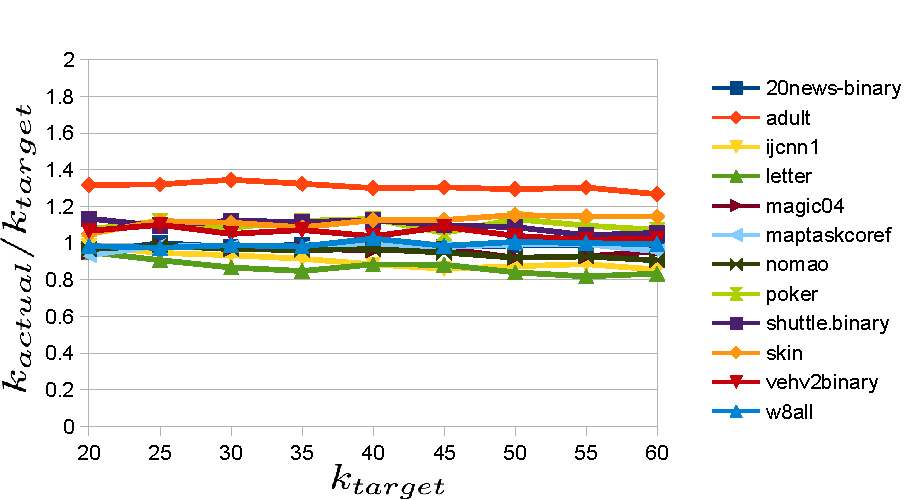
\includegraphics{figures/plot1.pdf}
\caption{The figure gives the ratio $k_{actual}/k_{target}$ on the $y$-axis as a function of $k_{target}$ on the $x$-axis.
The value $k_{target}$ is given to the algorithm as input and $k_{actual}$ is the resulting cardinality of the center set $C$.
We clearly see that this ratio is roughly constant and close $1$. Interestingly, the main differentiator is the dataset itself and not the value of $k_{target}$.
}
\label{fig1}
\end{center}
\end{figure}

\subsection{Online clustering cost}
Throughout this section, we measure the online $k$-means clustering cost with respect to different baselines. We report averages of at least 3 different independent executions for every parameter setting.
In Figure~\ref{fig2} the reader can see the online $k$-means clustering cost for the set of centers chosen online by our algorithm for different values of $k_{target}$ and different datasets.
For normalization, each cost is divided by $f_0$, the sum of squares of all vector norms in the dataset (akin to the theoretical $k$-means cost of having one center at the origin).
Note that some datasets are inherently unclusterable. Even using many cluster centers, the $k$-means objective does not decrease substantially.
Nevertheless, as expected, the $k$-means cost obtained by the online algorithm, $f_{online}$, decreases as a function of $k_{target}$. 

\begin{figure}[htbp]
\begin{center}
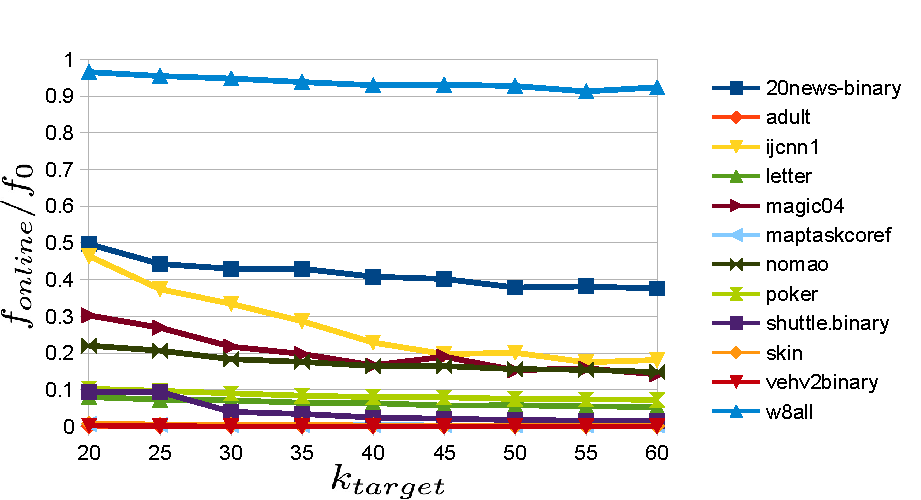
\includegraphics{figures/plot2.pdf}
\caption{Online $k$-means clustering cost ($f_{online}$) as a sanction of $k_{target}$ for the different datasets.
For normalization, each cost is divided by $f_0$, the sum of squares of all vector norms in the dataset (akin to the $k$-cost of once center in the origin).}
\label{fig2}
\end{center}
\end{figure}

The monotonicity of $f_{online}$ with respect to $k_{target}$ is unsurprising.
In Figure~\ref{fig3} we plot the ratio $f_{online}/f_{random}$ as a function of $k_{target}$.
Here, $f_{random}$ is the sum of squared distances of input points to $k_{actual}$  input points chosen uniformly at random (as centers).
Note that in each experiment the number of clusters used by the random solution and online $k$-means is identical, namely, $k_{actual}$.
Figure~\ref{fig3} illustrates something surprising. The ratio between the costs remains relatively fixed per dataset and almost independent to $k_{target}$.
Put differently, even when the $k$-means cost is significantly lower than picking $k$ random centers, they improve in similar rates as $k$ grows.

\begin{figure}[htbp]
\begin{center}
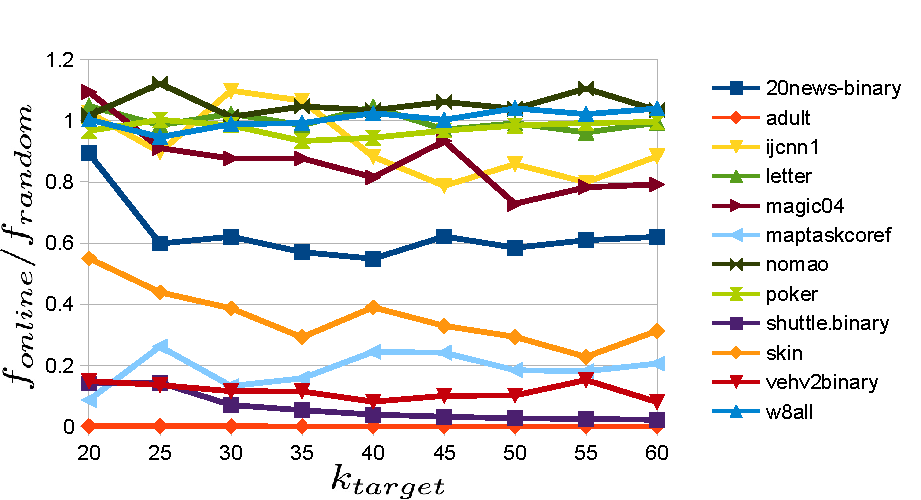
\includegraphics{figures/plot3.pdf}
\caption{On the $y$-axis, the value of $f_{online}$ divided by $f_{random}$. 
The latter is the cost of choosing, uniformly at random, as many cluster centers (from the data) as the online algorithm did.
A surprising observation is that this ratio is almost constant for each dataset and almost independent of $k_{target}$ (on the $x$-axis).}
\label{fig3}
\end{center}
\end{figure}

The next experiment compares online $k$-means to $k$-means++.
For every value of $k_{target}$ we ran online $k$-means to obtain both $f_{online}$ and $k_{actual}$.
Then, we invoke $k$-means++ using $k_{actual}$ clusters and computed its cost, $f_{kmpp}$.
This experiment was repeated $3$ times for each dataset and each value of $k_{target}$.
The mean results are reported in Figure~\ref{fig4}. 
Unsurprisingly, $k$-means++ is usually better in terms of cost. But, the reader should keep in mind that
$k$-means++ is an \emph{offline} algorithm that requires $k$ passes over the data compared with the online computational model of our algorithm.



\begin{figure}[htbp]
\begin{center}
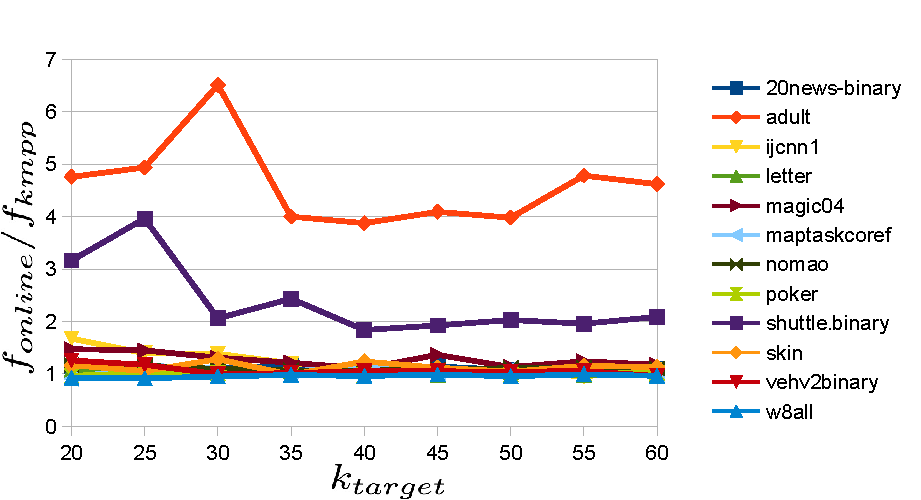
\includegraphics{figures/plot4.pdf}
\caption{On the $y$-axis we plot $f_{online}/f_{kmpp}$ as a function of $k_{target}$ on the $x$-axis. The values of $f_{online}$ is the cost of running Algorithm~\ref{alg2} with parameter $k_{target}$.
The value of $f_{kmpp}$ is the cost of running $k$-means++ with $k_{actual}$ clusters, $k_{actual}$ is the number of clusters online $k$-means actually used.
We see that, except for the datasets \emph{adult} and \emph{shuttle.binary}, $k$-means++ and online $k$-means are comparable. For \emph{adult} and \emph{shuttle.binary} online $k$-means is worse by a small constant factor. Note (Figure~\ref{fig3}) that both \emph{adult} and \emph{shuttle.binary} are datasets for which online $k$ means is dramatically better than random.}
\label{fig4}
\end{center}
\end{figure}

\begin{figure}[htbp]
\begin{center}
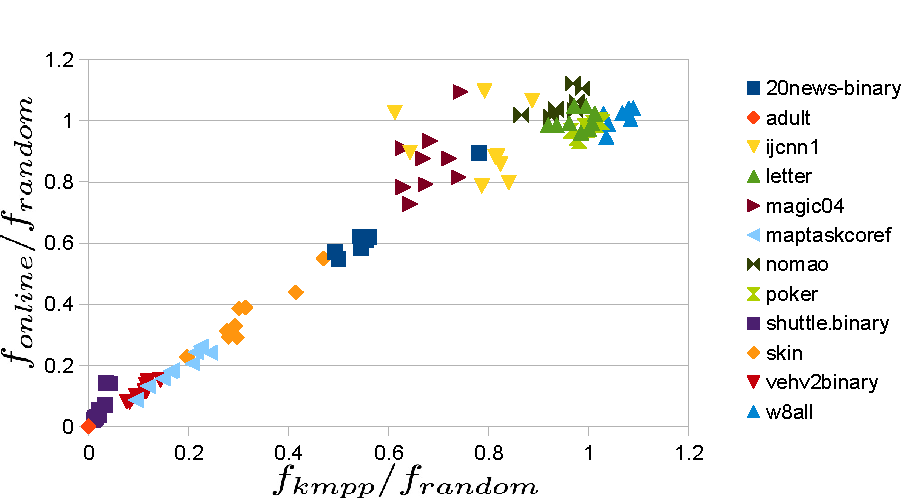
\includegraphics{figures/plot5.pdf}
\caption{On the $x$-axis $f_{kmpp}/f_{random}$ both using $k_{actual}$ clusters. 
The value of $k_{actual}$ is obtained by running online $k$-means with input $k_{target}$ on the $x$-axis.
The $y$-axis depicts $f_{online}/f_{random}$. 
Note that the performance of $k$-means++ and online $k$-means are very similar almost everywhere.
The advantage of $k$-means++ (see Figure~\ref{fig4}) occurs when the clustering cost is a minuscule fraction of random clustering.}
\label{fig5}
\end{center}
\end{figure}
  
\section{Aknowledgements}
We would like to thank  Dean Foster for  helping us with the proof of the Lemma \ref{random}.

\bibliographystyle{plain}
\bibliography{KMeans}





\appendix




\section{Online and Semi-Online Algorithms for $k$-means}\label{alg}

Our algorithm will run in phases, the phases will be indexed by $r\ge 1$. On each phase  let $f_r$ denote the parameter used as a cost gauge for opening a new cluster. Initially $f_1$ is defined to be the smallest non-zero squared distance between two vectors in our problem instance and $f_r=2\cdot f_{r-1}$ for $r\ge 2$.
The total number of demand points (or vectors) is $n$.  Each input vector is indexed by  $j=1,\dots,n$. 

When a new vector $v_j\in R^m$ arrives the algorithm either decides to put it into an existing cluster or opens a new cluster centered at $z=v_j$. For $j=1$ the algorithm always opens the first cluster centered at $v_1$.

When a new vector $v_j$ for $j\ge 2$ arrives, we run a generic step for the algorithm:

\begin{enumerate}
\item Let $C_1,\dots, C_q$ be the existing partition of the index set $\{1,\dots,j-1\}$ into clusters. Let $z_1,\dots,z_q$ be the corresponding cluster centers. Let $r\ge 1$ be the current phase of the algorithm. For each phase, let $q_r$ be the number of clusters opened during that phase. Note $q=\sum_{i=1}^rq_r$.
\item Compute $d^2_j$ the squared Eucledian distance from the nearest cluster center to $v_j$, let $i(j)$ be the index of  the closest cluster center. 
\item  Set
$$p=\min \left\{\frac{d^2_j}{f_r},1\right\}$$ and define a Boolean random variable $Q$ with $E[Q]=p$.
\item If $Q=1$ we  open a new cluster $C_{q+1}=\{v_j\}$ centered at $z_{q+1}=v_j$, increment $q=q+1$, $q_r=q_r+1$.  
\item If $Q=0$ we assign vector $v_j$ into the cluster indexed by $i(j)$, i.e. $C_{i(j)}=C_{i(j)}\cup \{v_j\}$.
\item 
\begin{enumerate}
\item In the semi-online algorithm: If $q_r\ge 3 k (1+ \log_2 n)$  we end the phase $r$ and move to the next one, i.e. $r=r+1$, the cluster cost is doubled and $q_{r}=0$.
\item In the fully online algorithm: If $q_r\ge 3 k(1+  \log_2 j)$  we end the phase $r$ and move to the next one, i.e. $r=r+1$, the cluster cost is doubled and $q_{r}=0$.
\end{enumerate}
\end{enumerate}



\end{document}


